\chapter[Metodologia]{Metodologia}
Este capítulo tem como objetivo apresentar a metodologia utilizada para desenvolvimento do TCC 1, e mostrar o plano base que servirá como guia para o desenvolvimento do TCC 2. A seção \ref{met_pesquisa} apresenta a classificação da metodologia utilizada para o desenvolvimento do trabalho. A seção \ref{met_desenvolvimento} descorre sobre o processo de desenvolvimento utilizado na criação da solução. E por último a seção  \ref{cronograma} apresenta o cronograma utilizado no desenvolvimento do TCC 1 é um cronograma para o TCC 2.
\section{Metodologia de Pesquisa}
\label{met_pesquisa}
Segundo \cite{moresi_metodologia_2003} a pesquisa pode ser entendida como um conjunto de ações que tem como objetivo encontrar um problema, construida através de procedimentos empíricos e sistemáticos. Para Moresi existem quatro classificações básicas para a pesquisa, quanto a sua natureza, sua abordagem, seu objetivo e o meio pelo qual é feita a investigação. A figura \ref{img:met_pesquisa} apresenta em quais características este trabalho se apresenta.
\graphicspath{{figuras/}}
\begin{figure}[h]
\centering
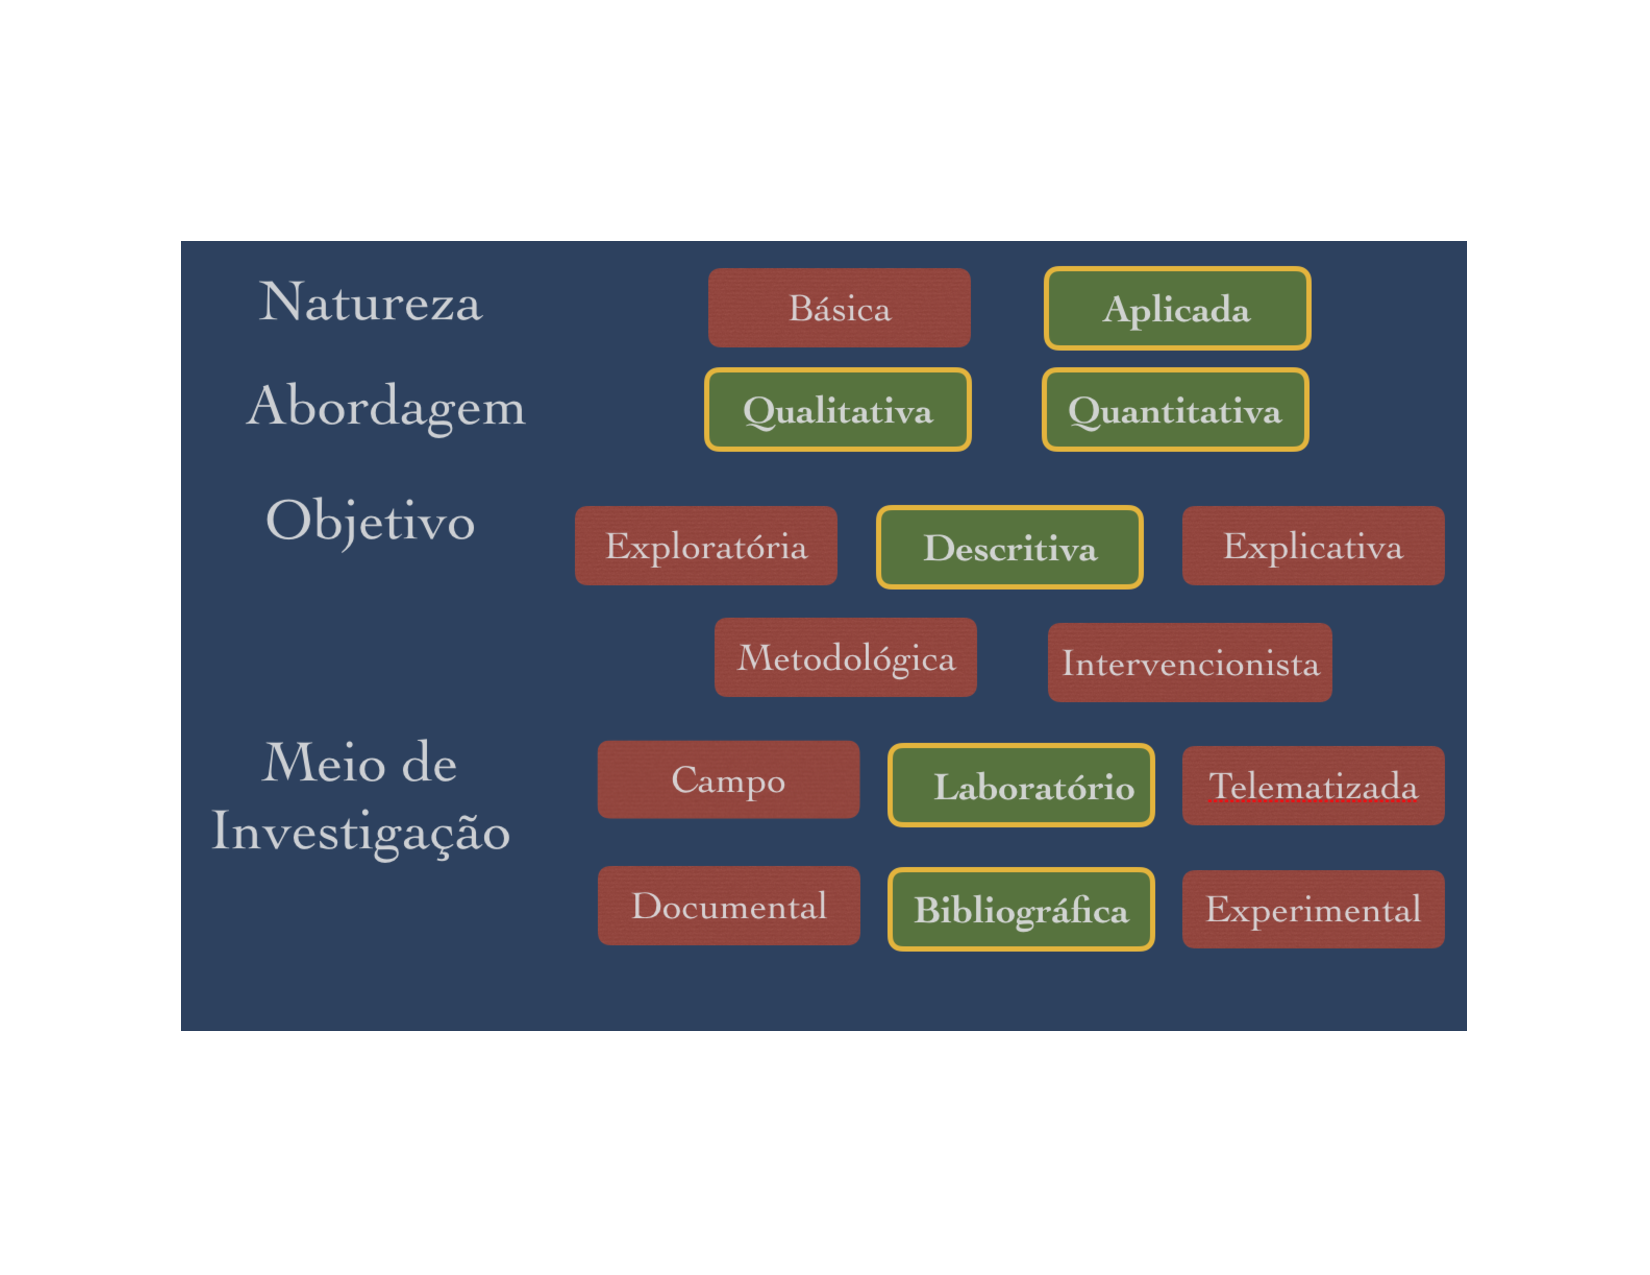
\includegraphics[scale=0.50]{metodologia_pesquisa}
\caption{Seleção das Características Metodológicas. Fonte: \cite{moresi_metodologia_2003}}
\label{img:met_pesquisa}
\end{figure}

Este trabalho tem um caráter mais voltado para uma pesquisa aplicada por envolver características espécificas na contratação de software do governo brasileiro. Outra característica que determina este trabalho como uma pesquisa aplicada é a natureza do trabalho estar voltado para o uso nas áreas de TI dentro dos orgãos públicos.
\\Segundo \cite{tatiana_denise} a pesquisa qualitativa é mais voltada para aspectos da realidade que não podem ser quantificados, mantendo o foco na compreensão. Neste aspecto o trabalho apresenta características qualitativas uma vez que a construção da solução é feita de maneira dinâmica se adaptando as necessidades do usuário. Segundo as autoras outra característica inerente a este tipo de pesquisa é a observação do mundo social ao mundo natural, está característica se apresenta de maneira muito forte quando propor a solução foi adotado um conjunto de métricas que são utilizadas no mercado ao invés de outros conjuntos apresentados por outros autores. 
\\Para Gil \cite{gil_como_2002} a pesquisa descritiva é focada em analisar características de uma população, fenômeno ou a relação entre as váriaveis as que compõem. Ests tipo de pesquisa não visa explicar os fenômenos que está descrevendo (apesar que a explicação para o fenômeno possa servir como base) \cite{moresi_metodologia_2003}. Este trabalho apresenta o caráter descritivo ao se tratar da natureza das contratações de software para orgão brasileiros, ou quando se fala de um processo de manutenção de software.
\\Por último o meio de investigação a ser aplicado é a pesquisa de campo. Moresi \cite{moresi_metodologia_2003} descreve a pesquisa de campo como sendo uma análise feita no local em que ocorre o fenômeno. Denise e Tatiana \cite{tatiana_denise} acrescentam que a pesquisa de campo além de analisar o local do fenômeno também realiza coleta dos dados. Por se tratar da implantação da solução em um orgão todo o acompanhamento da implantação será feito com base nas características deste órgão e a coleta dos dados será referente à este órgão. O fato de que a solução será utilizada em um ambiente real garante que aplicação não será utilizada em um ambiente controlado descartando a pesquisa laboratorial.
\\O plano metodológico consiste em duas fases iniciação e estudo da proposta. A primeira fase possui quatro atividades principais, são elas: Elaborar um roteiro de pesquisa, Pesquisar Referencias, Refinar Pesquisa e Catalogar material encontrado. Na atividade de elaboar um roteiro de pesquisa defini-se a string de busca e em quais bases serão pesquisados os materiais de referencia. A atividade de Pesquisar referencias como o próprio nome ja sugere envolve a pesquisa da string de busca nas bases selecionadas. Refinar pesquisa envolve elaborar uma nova string de busca que contenha termos mais especificos e que aumente a quantidade de arquivos referentes ao tema. Catalogar material é uma atividade focada em guardar os materiais encontrados colocando uma tag referente ao tema a que o artigo se refere e uma breve descrição sobre o que era mais importante. 
\\A Segunda fase consiste em estudar o cenario em que será colocado a dashboard para que se possa entender quais as necessidades e os requisitos para implantação. Esta fase está dividida em três momentos: planejar,  executar e checar. Durante o momento de planejar tem-se como principais atividades analisar o problema onde há um maior entendimento do contexto no qual será elaborado a solução. A segunda atividade é elaborar solução em que é esperado que ao fim dessa atividade exista um esboço do que será a solução final. No segundo momento implementa-se a solução e no terceiro momento acontece a validação dessa solução.
\graphicspath{{figuras/}}
\begin{figure}
\centering
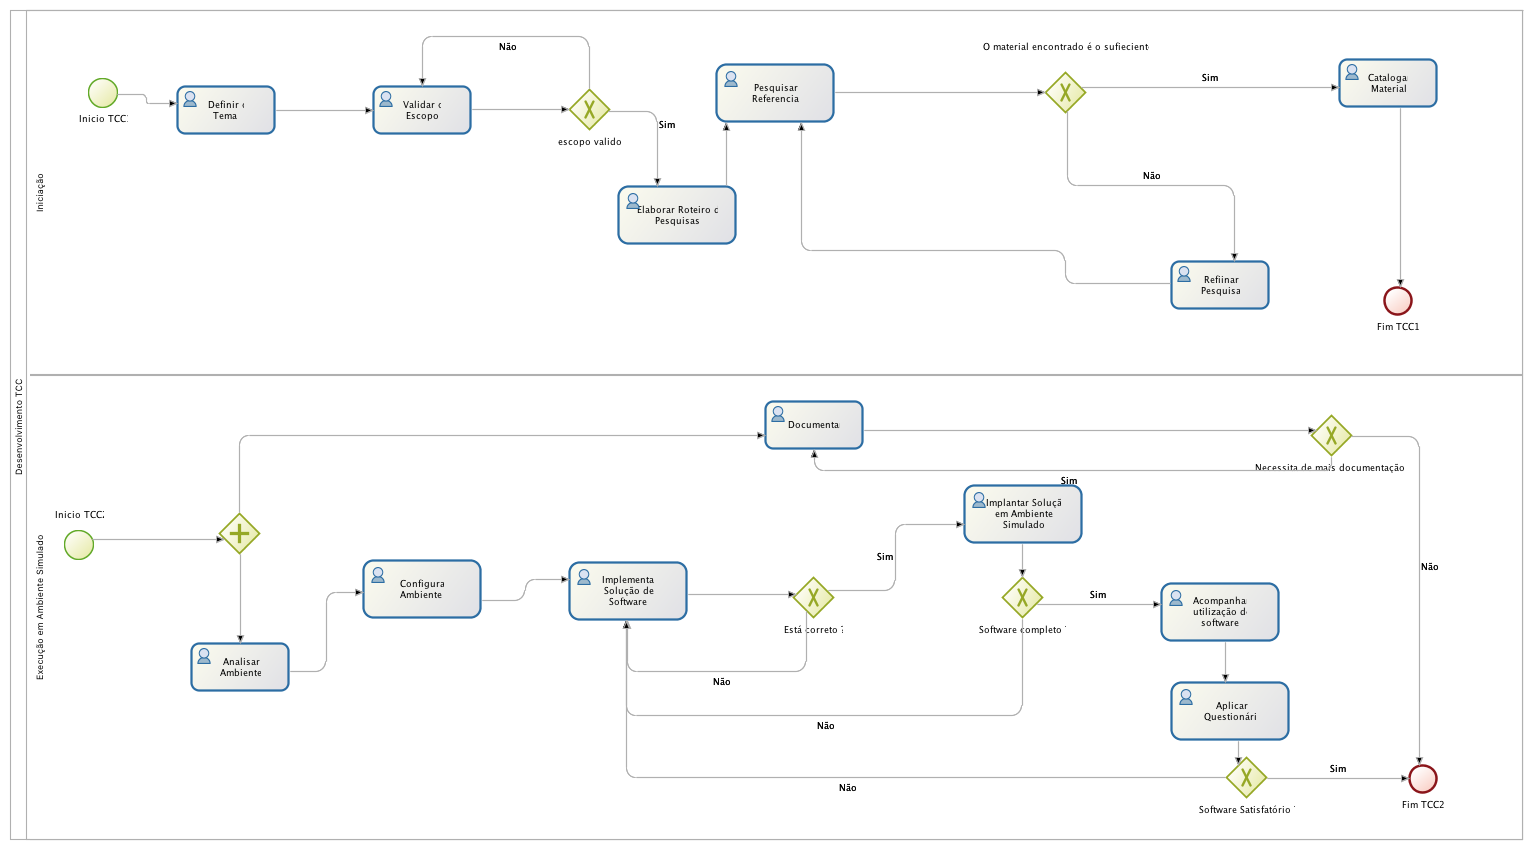
\includegraphics[scale=0.40]{TCCMetodologia}
\caption{Plano de Pesquisa}
\label{Rotulo}
\end{figure}

\section{Metodologia de Desenvolvimento}
\label{met_desenvolvimento}
O dashboard será criado utilizando de uma adaptação da metodologia de desenvolvimento Scrum. Os principais conceitos que foram utilizados da metodologia foram:
\begin{itemize}
\item \textit{\textbf{Product Backlog}}: Lista de atividades que representam as funcionalidades que serão construidas no projeto. O \textit{Product Owner} é quem escreve o \textit{product backlog}, essas atividades são mutáveis ao decorrer do projeto, pois a equipe de desenvolvimento acaba conhecendo mais do produto \cite{sabbagh_scrum:_2014}.
\item \textit{\textbf{Sprint}}: Ciclo de desenvolvimento com prazo definido em que são desenvolvidas as atividades do projeto. Neste trabalho definiu-se como sendo 15 dias o período referente a uma \textit{Sprint}
\item \textit{\textbf{Sprint Backlog}}: Atividades referentes à uma determinada \textit{Sprint} na qual a equipe de desenvolvimento se compromete a entregar. Estas atividades são retiradas do \textit{product backlog} \cite{mahnic_case_2011}.
\item \textbf{História do Usuário}: Descrição do ponto de vista do usuário sobre uma funcionalidade do produto. Este artefato é composto do que é conhecido como 3C's, Cartão, Conversa e Confirmação. O cartão é referente ao fato de se documentar a conversa em um cartão, este sendo acessível a todo o time de desenvolvimento. A conversa é uma breve descrição da funcionalidade sob o olhar do usuário, um exemplo pode ser observado na figura \ref{img:us}. E a confirmação ou critérios de aceitação é um \textit{checklist} abordando o que deve ser verificado para que a história seja dada como concluida.
\graphicspath{{figuras/}}
\begin{figure}[h]
\centering
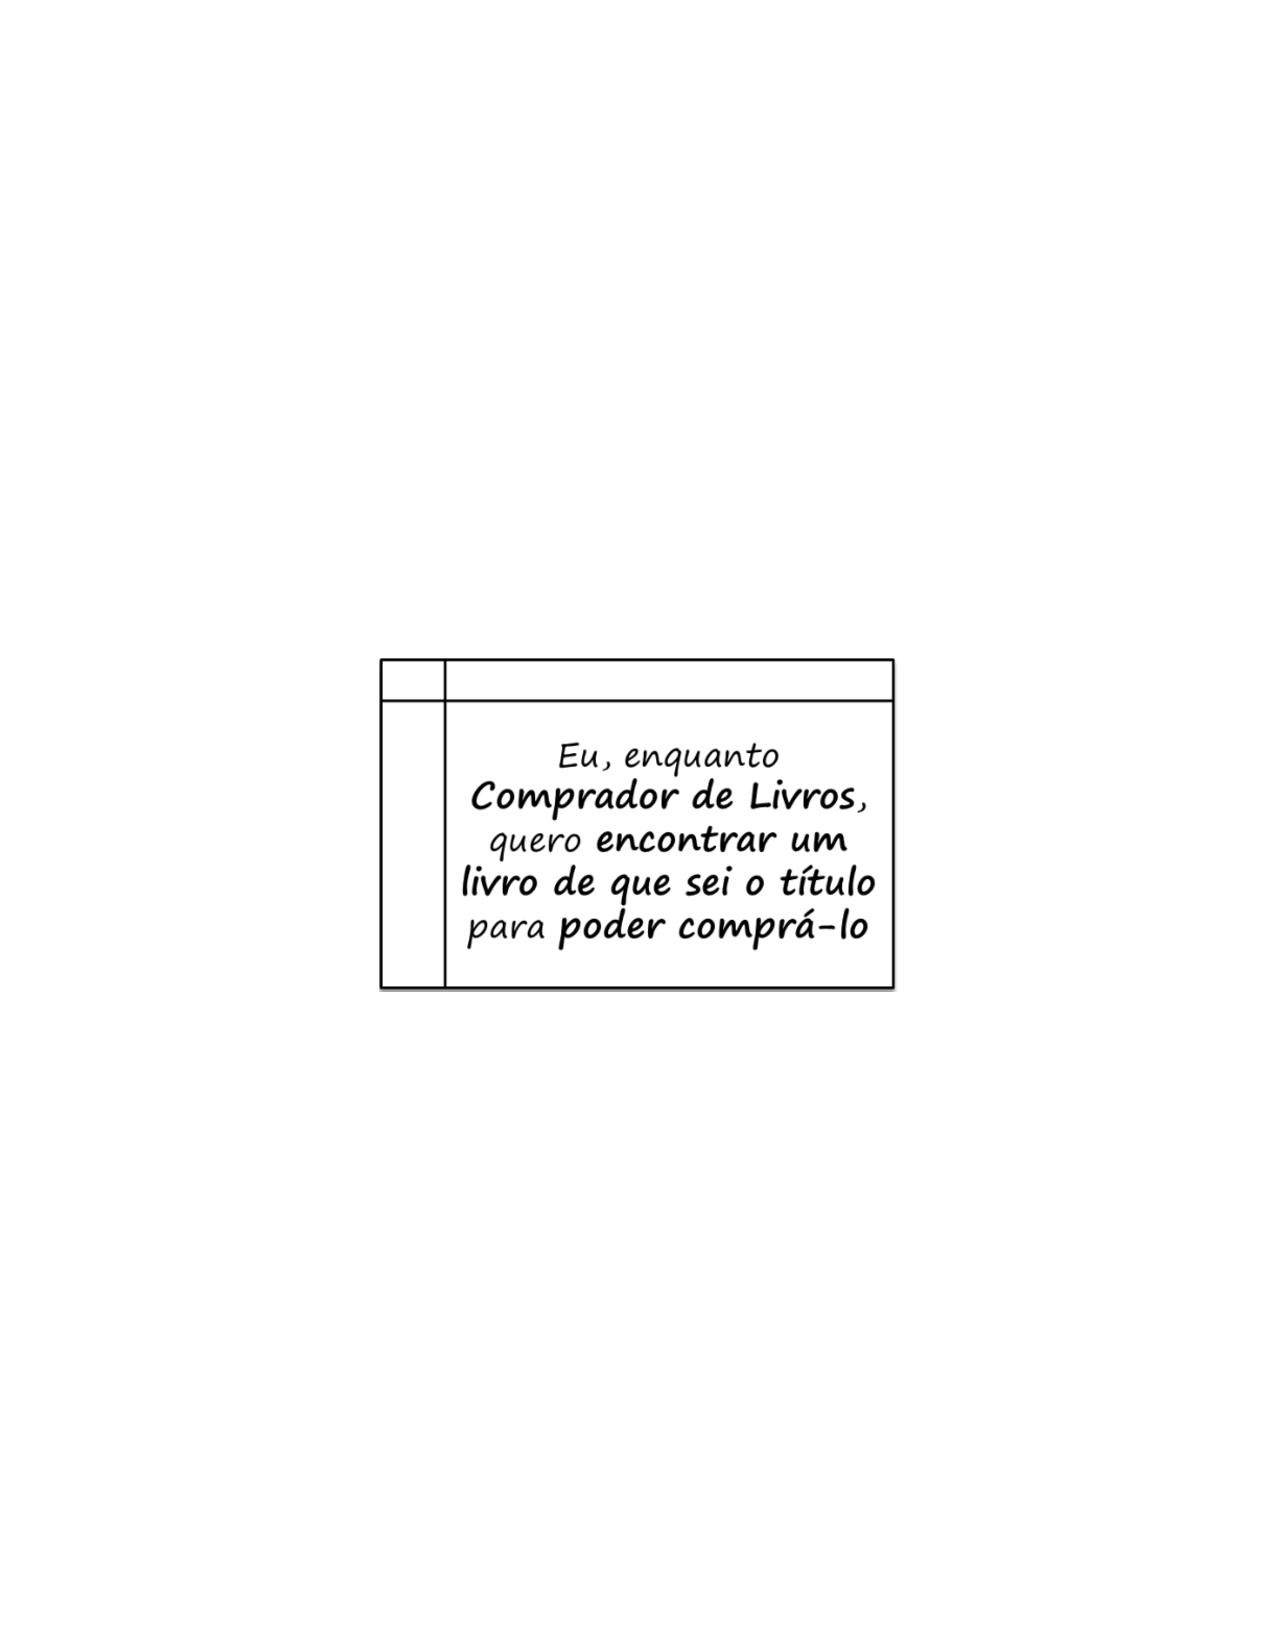
\includegraphics[scale=0.80]{US}
\caption{Exemplo de História de Usuário. Fonte: \cite{sabbagh_scrum:_2014}}
\label{img:us}
\end{figure}
\item \textit{\textbf{Story Point}}:Unidade relativa que caracteriza o esforço da equipe de desenvolvimento para finalizar uma atividade. A escala utilizada é definida pela equipe de desenvolvimento, neste trabalho será utilizado a escala de Fibonacci (1,2,3,5,8,13, ...). 
\end{itemize}
\section{Cronograma}
\label{cronograma}
\begin{table}[http]
	\centering
	\caption{Cronograma TCC 1}
	\label{tab:cronograma}
	\begin{tabular}{ccccc}
		\hline
		\multicolumn{1}{|c|}{\textbf{Cronograma}}             & \multicolumn{1}{c|}{\textbf{Agosto}} & \multicolumn{1}{c|}{\textbf{Setembro}} & \multicolumn{1}{c|}{\textbf{Outubro}} & \multicolumn{1}{c|}{\textbf{Novembro}} \\ \hline
		\multicolumn{1}{|c|}{Realizar Pesquisa Bibliográfica} & \multicolumn{1}{c|}{X}              & \multicolumn{1}{c|}{X}              & \multicolumn{1}{c|}{X}             & \multicolumn{1}{c|}{X}              \\ \hline
		\multicolumn{1}{|c|}{Estudar o orgão}             & \multicolumn{1}{c|}{}               & \multicolumn{1}{c|}{X}              & \multicolumn{1}{c|}{X}             & \multicolumn{1}{c|}{}               \\ \hline
		\multicolumn{1}{|c|}{Propor Versão Inicial do dashboard}                & \multicolumn{1}{c|}{}               & \multicolumn{1}{c|}{}               & \multicolumn{1}{c|}{X}             & \multicolumn{1}{c|}{X}              \\ \hline
		\multicolumn{1}{l}{}                                  & \multicolumn{1}{l}{}                & \multicolumn{1}{l}{}                & \multicolumn{1}{l}{}               & \multicolumn{1}{l}{}                \\
		\multicolumn{1}{l}{}                                  & \multicolumn{1}{l}{}                & \multicolumn{1}{l}{}                & \multicolumn{1}{l}{}               & \multicolumn{1}{l}{}                \\
		\multicolumn{1}{l}{}                                  & \multicolumn{1}{l}{}                & \multicolumn{1}{l}{}                & \multicolumn{1}{l}{}               & \multicolumn{1}{l}{}               
	\end{tabular}
\end{table}
